\chapter{The influence of galaxy environment}\label{chap:env}
 
So far, I have considered  galaxy mergers \& interactions, morphology and AGN as possible causes of quenching across the galaxy population. While it is abundantly clear that these processes can strongly affect the SFHs of galaxies, the density of a galaxy's environment is also thought to be a driver of galaxy evolution (see Section~\ref{sec:quenchmech}).
 
The galaxy environment as a driver of quenching was proposed due to the correlation of environmental density with morphology \citep{dressler80, smail97, poggianti99, postman05, Bamford09}, colour \citep{butcher78, pimbblet02} and the quenched galaxy fraction \citep{kauffmann03, Baldry06, peng12, darvish16}. Star forming disc galaxies tend to be located in low-density environments with quiescent elliptical galaxies in more dense environments. Although these correlations were originally interpreted as indicating causation, recent evidence from simulations suggests that quenching mechanisms driven by the environment may not be dominant in the galaxy lifecycle \citep{kimm09, kimm11, hirschmann14, wang14, phillips15}. Perhaps, instead, the correlation of increased quenched galaxy fractions with environment density is due to a superposition of the effects of mergers, interactions and both mass and morphology quenching. 
  
In order to isolate the cause of the density-morphology and density-SFR correlations, I need to observe how morphology and galaxy quenching timescales change in dense environments with different properties in comparison to the field. Here, I consider the group environment, as this is a more typical environment for a galaxy than the relatively rare rich cluster environment \citep{carlberg04}. I construct a sample of both group and field galaxies and once again use \starpy\ to determine the quenching time and rate to describe a simple SFH for a galaxy given its photometry. However, dense environments are messy with many possible mechanisms at work, whose effects are difficult to disentangle. %The effects of these various mechanisms would be washed out across the population density distributions produced by \textsc{popstarpy} and so I do not employ this method in this Chapter. Instead, I will simplify my analysis in order to separate the effects of the different quenching mechanisms contributing to the galaxy population in the group environment (see Section~\ref{sec:delta}). 

I aim to determine the following: (i) How does the environment influence the detailed morphological structures of a galaxy?  (ii) Is quenching which is directly caused by the environment occurring in galaxy groups?
 
 
%In Section~\ref{sec:data} I describe the group catalogue employed and highlight the results in Section~\ref{sec:results}. 
 
\section{Data and Methods}\label{sec:data}

\subsection{Group Identification}\label{sec:groups}

The construction of a robust cluster or group catalogue is a thesis in itself, with many studies attempting this across the SDSS \citep{merchan05, miller05, berlind06, yang07, tago08, tago10, tinker11, munoz12, tempel14} and other large surveys \citep{tucker00, merchan02, eke04, cucciati10, robotham11, knobel12}. The difficulties arise in removing projection effects, understanding the selection function used, covering large ranges in mass and redshift, and dealing with spectral fibre collisions (see the comprehensive review by \citet{postman02} for an in depth discussion). Various different methods have been employed to achieve robust cluster/group identification including clustering algorithms \citep[e.g.][]{miller05}, galaxy colour modelling \citep{koester07}, adaptive filter halo modelling \citep{yang05, yang07} and friends-of-friends algorithms \citep{goto05, merchan05, berlind06}. 

Each group finding algorithm has to be tested for purity (how contaminated the groups are by non-members) and completeness (how often are true members excluded from a group). \citet{campbell15} compared the purity and completeness of two of the most frequently used group catalogues of \citet[][a friends-of-friends algorithm]{berlind06} and \citet[][a halo modelling algorithm]{yang07} and concluded that no sample could achieve perfect purity or completeness. Despite the different algorithms employed to identify group galaxies, \citeauthor{campbell15} found that the two catalogues are remarkably similar. The \citeauthor{yang07} catalogue has however, higher purity of satellites at lower halo masses (i.e. the low halo mass groups are less contaminated by non-members). For this reason the \citeauthor{yang07} catalogue is the most commonly used in environment studies using data from the SDSS \citep[including][]{hoyle11, pasquali12, wetzel14, shankar14, lacerna14, knobel15, fitzpatrick15, lan16, woo16, bluck16, weigel16}, but I find that when cross matched with the \textsc{gz2-galex} sample (with a $3''$ search radius) only $38$ galaxies (of $176,604$ possible galaxies) which belong to a group with 2 or more members are identified. This is most likely due to the necessity for GALEX NUV photometry in this study. The majority of NUV emission comes from massive, short lived stars and so in the cluster environment which is dominated by typical `red and dead' quiescent galaxies, detecting NUV emission is less likely. 

Consequently I use the \citet{berlind06} catalogue, which when cross matched with the \textsc{gz2-galex} sample and limited to $z < 0.1$\footnote{To ensure GALEX completeness of the red sequence, unlike in Chapter~\ref{chap:morph}; see \citealt{Wyder07, Yesuf14}}, gives $14,199$ group galaxies with the number of group members, $N_{\rm{group}} \geq 2$. Centrals were selected as the most massive galaxy in a group \citep[as in][]{yang07, yang09, pasquali10} with all other galaxies in a group designated as satellites.

The projected group-centric radius, $R$, of all satellite galaxies was calculated from the projected separations of the co-ordinates of a satellite from its central; this was then converted to $\rm{kpc}$ by using the observed spectroscopic redshift of the central galaxy. In order to compare groups of different sizes, the virial radius is used as a normalisation factor to this projected group-centric radius. Here I use a proxy to the virial radius, $R_{200}$\citep[see][]{navarro95}, the radius within which the group mass overdensity is 200 times the critical density, $\rho_{\rm{crit}}(z)$, as defined by \citealt{finn05}:
\begin{equation}\label{eq:overdense}
200\rho_{\rm{crit}}(z) = \frac{M_{cl}}{\frac{4}{3}\pi R_{200}^3},
\end{equation}

where $M_{cl}$ is the mass of the group. \citeauthor{finn05} then use the redshift dependence of the critical density and the virial mass to relate the line-of-sight velocity dispersion, $\sigma_x$, to the group mass so that $R_{200}$ becomes:
\begin{equation}\label{eq:r200}
R_{200} = 1.73 \left ( \frac{\sigma_x}{1000 \rm{km}~\rm{s}^{-1}} \right) \cdot \frac{1}{\sqrt{\Omega_{\Lambda} +\Omega_o(1+z)^3}} ~ h_{100}^{-1} ~\rm{Mpc}, 
\end{equation}

$\sigma_x$ is calculated for a group as the standard deviation of the velocity dispersions $\sqrt{(v_i - \left< v_i\right>)^2}$. Here $v_i$ are the proper velocities of each galaxy, $i$, as defined in \cite{danese80}:
\begin{equation}\label{eq:propervel}
v_i = c \cdot \frac{z_i - z_{group}}{1 + z_{group}},
\end{equation}
where $z_{group}$ is the mean redshift of all the group members. Since most groups in the sample have low $N_{\rm{group}}$, using the mean redshift for $z_{\rm{group}}$, rather than the central galaxy redshift is most appropriate in this case. These calculations resulted in a sample of $3,468$ centrals and $10,731$ satellites within a projected group-centric radius range of $0.02 < R/R_{200} < 24.9$ and $z < 0.084$ which shall be referred to as the \textsc{gz2-berlind} sample. Note that for a galaxy (central or satellite) to be included in the \textsc{gz2-berlind} sample, the rest of its group does not. However the properties of that group are still retained by the included galaxy. 

Unlike in previous Chapters, here I will specifically focus on galaxies that are below the star forming sequence (SFS) in order to simplify the analysis (see Section~\ref{sec:resultssfhs}). I therefore select a subsample of the \textsc{gz2-berlind} galaxies that are $1\sigma$ below the SFS, giving $4,629$ satellite and $2,314$ central galaxies which will collectively be referred to as the \textsc{gz2-group} sample. These galaxies are shown in the panels of Figure \ref{fig:sfrmass} and can be seen to lie below the SFS.

\begin{figure}
\centering
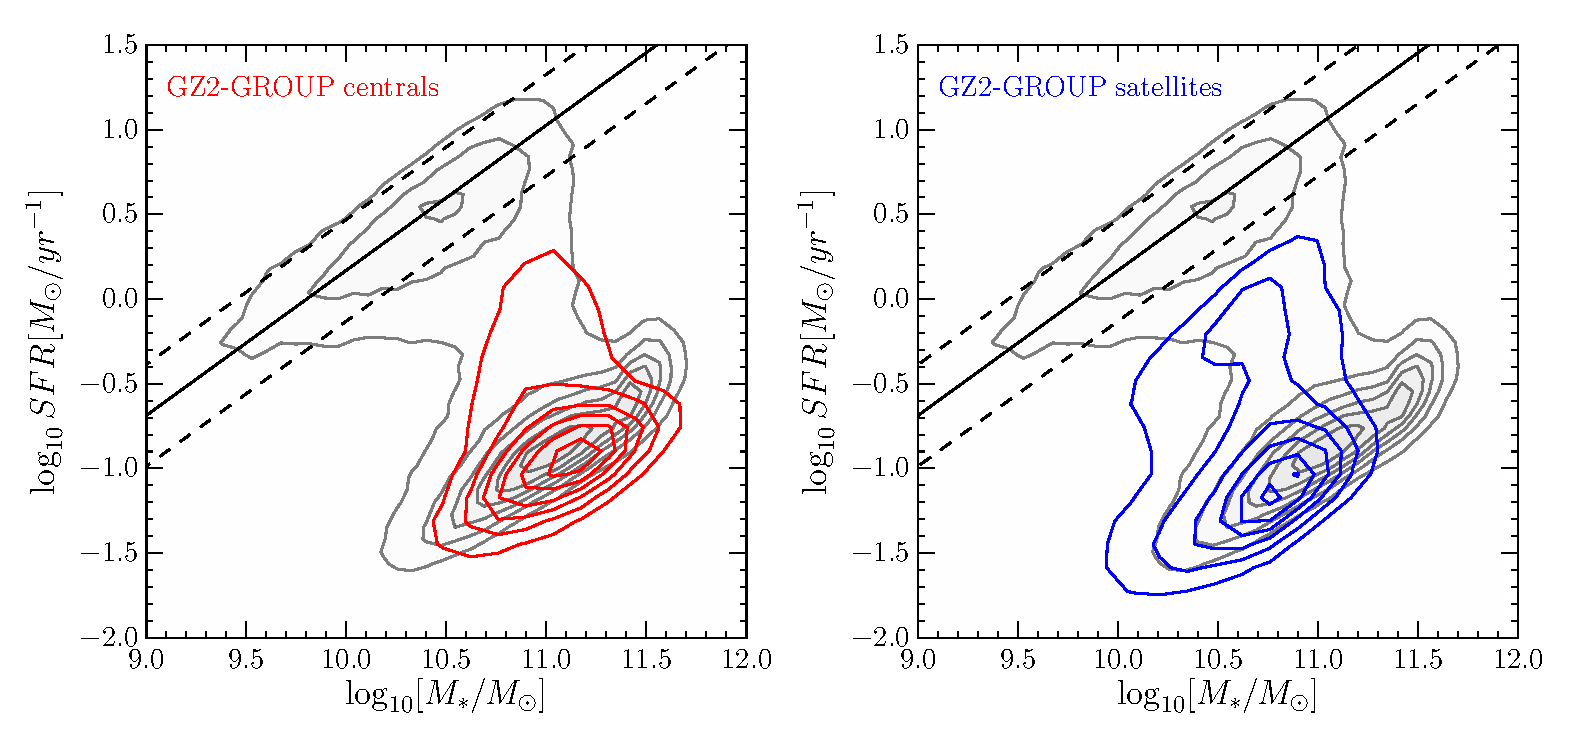
\includegraphics[width=\textwidth]{environment/sfr_mass_quenched_centrals_satellites_gz2_group.pdf}
\caption[Stellar mass-SFR plane for the centrals and satellites of the \textsc{gz2-group} sample]{The stellar mass-SFR plane showing central (left; red contours) and satellite (right; blue contours) in the \textsc{gz2-group} sample. In both panels the entire SDSS sample from the MPA-JHU catalogue is shown by the grey contours. The definition of the SFMS from \cite{peng10} at $\overline{z} = 0.053$ (solid line, the mean redshift of the \textsc{gz2-group} sample) with $\pm1\sigma$ (dashed lines) is shown.}
%KS Test between distributions?
\label{fig:sfrmass}
\end{figure}


I also compare the \textsc{gz2-berlind} and \textsc{gz2-group} samples with a measurement of the projected neighbour density from \cite{Baldry06}, $\Sigma_N = N/4\pi d_N^2$, where $d_N$ is the distance to the $N^{\rm{th}}$ nearest neighbour. $\Sigma$ is a more direct probe of the local density of a galaxy's environment, and although it does not allow for the identification of groups and their properties, it is still a useful probe of the local density inside a group  \cite[see][for a comparison of various environment parametrisations]{muldrew12}.

In this work I use the estimates of \cite{Bamford09} who calculated the local galaxy density, $\Sigma$, determined by averaging $\log\Sigma_N$ for $N = 4$ and $N=5$ by the method outlined in \citet{Baldry06}, for the entirety of the GZ1 sample. $90\%$ of the \textsc{gz2-berlind} sample have $\log\Sigma > -0.8$ (the threshold quoted by \citealt{Baldry06} to define non-field galaxies), suggesting a purity of $\sim90\%$ for the \textsc{gz2-berlind} sample. The distributions of $\log\Sigma$ for star forming and quenching/quenched centrals and satellites in the \textsc{gz2-berlind} sample are shown in Figure~\ref{fig:sigmadist}. Star forming galaxies tend to reside in less dense local environments than their quenching or quenched counterparts. The satellite galaxies as a whole also seem to occupy denser local environments than centrals, however on investigation this seems to arise because the satellites in the \textsc{gz2-berlind} sample reside in groups with larger $N_{group}$ than the centrals. This is to be expected given the definition of a satellite galaxy. 

\begin{figure}
\centering
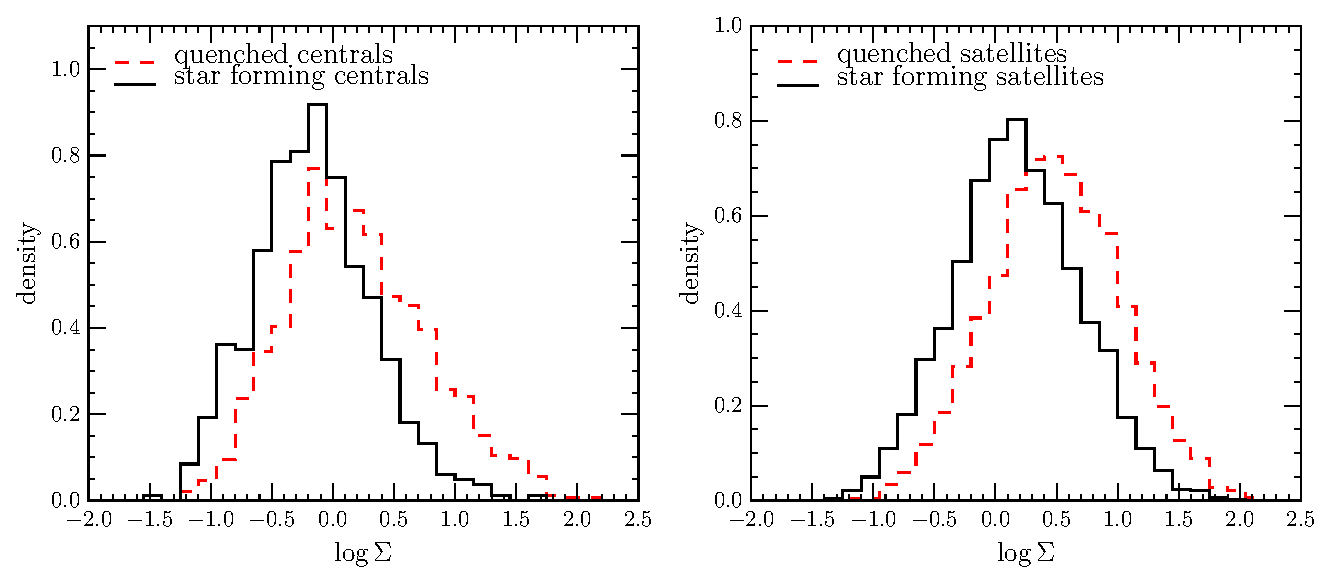
\includegraphics[width=\textwidth]{environment/SIGMA_density_sf_q_cent_sat.pdf}
\caption[Local environment density distributions of central and satellite galaxies]{Local environment density, $\log\Sigma$, distributions of star forming (black) and quenching/quenched (red) central (left) and satellite (right) galaxies in the \textsc{gz2-group} sample.}
%KS Test between distributions?
\label{fig:sigmadist}
\end{figure}


\subsection{Field sample}\label{sec:field}

I constructed a sample of field galaxies for use as a control sample to the \textsc{gz2-group} sample. For all galaxies in the \textsc{gz2-galex} sample, I calculated the smallest projected group-centric radii, $R/R_{200}$, from each of the central galaxies in the \citet{berlind06} catalogue (regardless of whether the central was included in the \textsc{gz2-berlind} sample) and selected candidate field galaxies as those with (i) $R/R_{200} > 25$ and (ii) $\log\Sigma < -0.8$ \citep[the threshold on the local environment density which selects field galaxies as defined by][]{Baldry06}. I chose to use both of these environmental density measures to ensure a pure sample of candidate field galaxies.

This sample of field galaxy candidates was then matched in redshift and stellar mass firstly to the central galaxies of the \textsc{gz2-group} sample to give $2,309$ field galaxies with $z < 0.084$. In this work I shall focus on galaxies which are either quenching or quenched and are more than $1\sigma$ below the SFS (as defined in \citet{peng10}, see Section~\ref{qmod}) and so the same constraints must be placed on this field control sample. This encompasses $1,596$ field galaxies with $z < 0.084$ which will be referred to as the \textsc{gz2-cent-field-q} sample. It will be used as a control sample when investigating the trends with central galaxy properties of the inferred quenching parameters. The redshift distribution of the \textsc{gz2-cent-field-q} sample is shown in comparison to the distribution of central galaxies in the \textsc{gz2-group} sample in the left panel of Figure~\ref{fig:zcompare}. %SDSS images of a random selection of galaxies from the \textsc{gz2-group} and \textsc{gz2-cent-field-q} samples are shown ordered by their GZ2 debiased vote fraction in Figure~\ref{fig:mosaic}. %KS test between samples?

Secondly, the field galaxy candidates were matched in redshift and stellar mass to the satellite galaxies of the \textsc{gz2-group} sample to give $5, 004$ field galaxies with $z < 0.084$ which will be referred to as the \textsc{gz2-sat-field} sample. These galaxies will be used as a control when investigating the morphological trends of satellite galaxies with environment. Note that this sample is not restricted to being $1\sigma$ below the SFS. $237$ galaxies are found in both the \textsc{gz2-cent-field-q} and \textsc{gz2-sat-field} samples. The redshift distribution of the \textsc{gz2-sat-field} sample is shown in comparison to the distribution of satellite galaxies in the \textsc{gz-group} sample in the right panel of Figure~\ref{fig:zcompare}.

We obtain SFRs and stellar velocity dispersions of galaxies for all of the field samples described above from the MPA-JHU catalogue \citep{kauffmann03, brinchmann04}. Stellar masses were already calculated for the entire \textsc{gz2-galex} sample using the optical photometry and the method outlined in \citet{Baldry06} (see Section~\ref{sec:defsample}).

\begin{figure}
\centering{
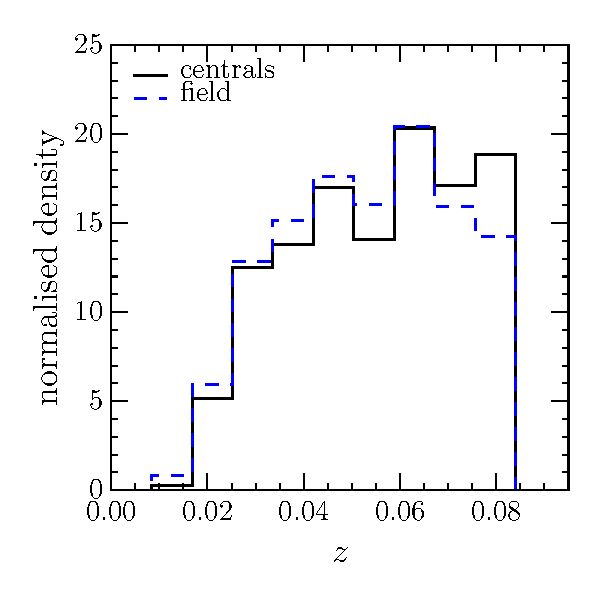
\includegraphics[width=0.45\textwidth]{environment/redshift_cent_field.pdf}
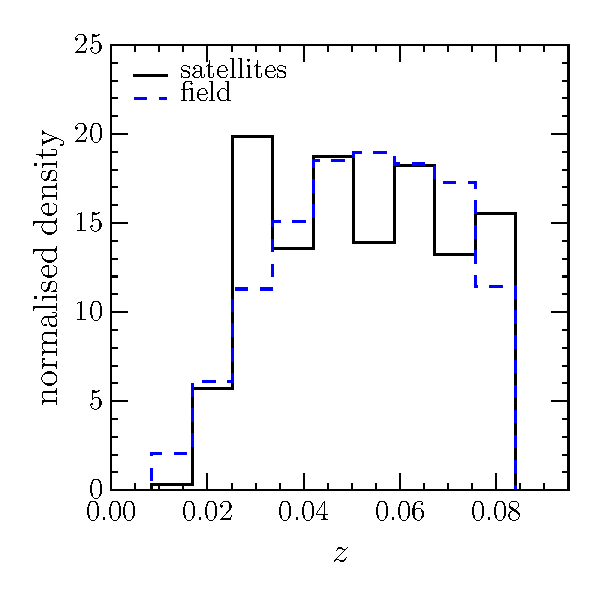
\includegraphics[width=0.45\textwidth]{environment/redshift_sat_field.pdf}}
\caption[Redshift distribution of galaxies in the \textsc{gz2-group} sample]{Redshift distributions of central (left) and satellite galaxies (right) in the \textsc{gz2-group} sample (black solid line) in comparison the redshift matched \textsc{gz2-cent-field-q} (left; blue dashed line) and \textsc{gz2-sat-field} samples (right; blue dashed line).}
%KS Test between distributions?
\label{fig:zcompare}
\end{figure}

\subsection{Morphological fractions}\label{sec:morphfrac}

I once again utilise the GZ2 vote fraction to quantify the morphology of galaxies in the \textsc{gz2-group} sample, in order to investigate the morphological trends with group radius. As in previous Chapters, I shall utilise $p_{\rm{disc}}$ and $p_{\rm{smooth}}$ but will also use $p_{\rm{bar}}$, $p_{\rm{bulge}}$ and $p_{\rm{merger}}$ to calculate the bar, bulge and merger fractions in the \textsc{gz2-group} sample respectively. 

Fractions are calculated considering the number of barred (with $p_{\rm{bar}} > 0.5$; see \citealt{masters11a, Cheung13}) and bulged (with $p_{\rm{obvious}~\rm{or}~\rm{dominant}} > 0.5$ and $p_{\rm{none}~\rm{or}~\rm{noticeable}} > 0.5$ from Task 4 in the GZ2 decision tree shown in Figure~\ref{fig:gztree}) galaxies over the number of disc galaxies ($p_{\rm{disc}} > 0.43$, $p_{\rm{edge\_on, no}} > 0.715$, $N_{\rm{edge\_on, no}} > 20$; see Table~\ref{table:votes} in Chapter~\ref{chap:intro}) in the \textsc{gz2-group} satellite sample. The merger fraction considers the number of merging galaxies (with $p_{\rm{merger}} > 0.4$; see \citealt{Darg10a}) over the number of galaxies in the \textsc{gz2-group} satellite sample. 

\section{Results}\label{sec:results}

\subsection{Mass dependence with radius}

Since morphological features have been shown to be dependent on the stellar mass of a galaxy \citep[e.g. the increase in the bar fraction with stellar mass; see][]{nair10, skibba12}, before investigating trends in the morphology with group radius in the \textsc{gz2-group} sample, the mass dependence on the group radius must be considered. This is shown in Figure~\ref{fig:massdep}. The mean stellar mass is roughly flat and consistent with the median field value with increasing group radius, until the most central group radius bin at $R \sim 0.1~R_{200}$. This trend is present for both morphologies, with early-type galaxies showing a larger increase in the average stellar mass. I note that if this inner bin at $0.1 R/R_{200}$ is ignored in the results that follow, my conclusions still hold. 

\begin{figure}
\centering{
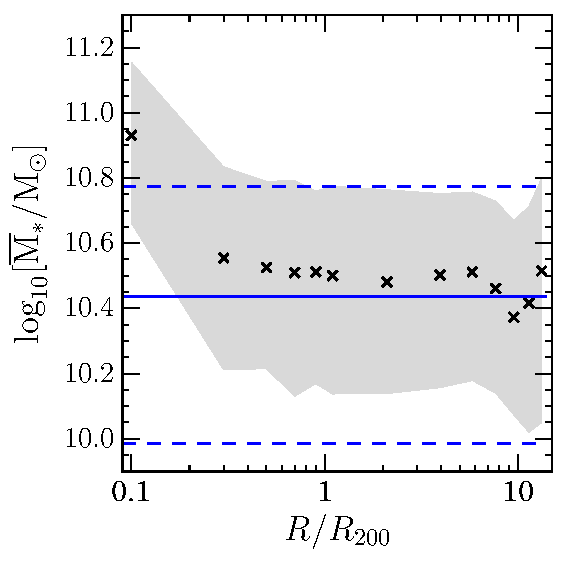
\includegraphics[width=0.45\textwidth]{environment/mass_trend_with_log_radius_compare_field.pdf}}
\caption[Average mass with group radius in the \textsc{gz2-group} sample]{The average stellar mass as a function of radius from the group centre. The shaded regions show the $\pm1\sigma$ in each bin of $R/R_{200}$. The average stellar mass of the \textsc{gz2-sat-field} sample is also shown (blue solid line) with $\pm1\sigma$ (blue dashed line).}
\label{fig:massdep}
\end{figure}



\subsection{Dependence of detailed morphological structure with environment}\label{sec:resmorph}

\begin{figure}
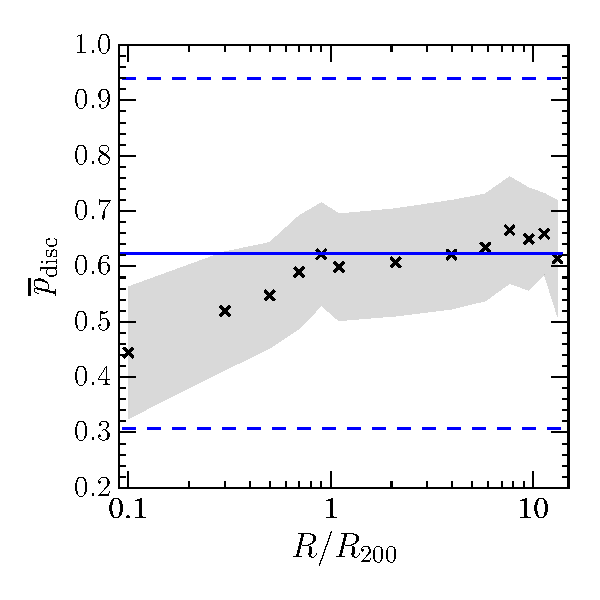
\includegraphics[width=0.46\textwidth]{environment/p_disc_trend_with_log_radius_field_compare.pdf}
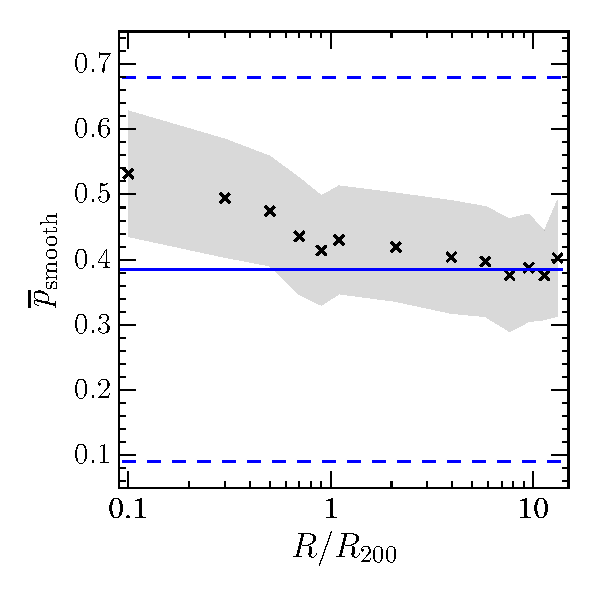
\includegraphics[width=0.46\textwidth]{environment/p_smooth_trend_with_log_radius_field_compare.pdf}
\caption[Mean $p_d$ and $p_s$ with group radius in the \textsc{gz2-group} sample]{Mean GZ2 vote fraction for disc (left) and smooth (right) galaxies in the \textsc{gz2-group} sample binned by projected group-centric radius, normalised by $R_{200}$, a proxy for the virial radius of a group. The shaded region shows $\pm1\sigma$ on the mean vote fraction. The mean vote fraction of the \textsc{gz2-sat-field} sample are also shown (blue solid lines) with $\pm1\sigma$ (blue dashed lines).}
\label{fig:morphradius}
\end{figure}

\begin{figure}
\centering{
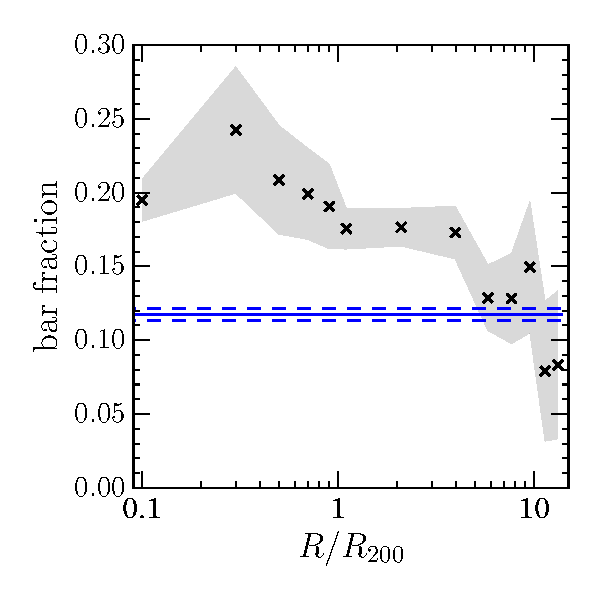
\includegraphics[width=0.46\textwidth]{environment/bar_fraction_over_disc_trend_with_log_radius_sat_matched_field_cand.pdf}}
\caption[Bar fraction with group radius in the \textsc{gz2-group} sample]{Bar fraction (number of barred disc galaxies over number of disc galaxies) in the \textsc{gz2-group} sample binned in projected group-centric radius, normalised by $R_{200}$, a proxy for the virial radius of a group. The shaded region shows $\pm1\sigma$ on the bar fraction. The bar fraction of the \textsc{gz2-sat-field} sample is also shown (blue solid line) with $\pm1\sigma$ (blue dashed line).}
\label{fig:barradius}
\end{figure}

\begin{figure}
\centering{
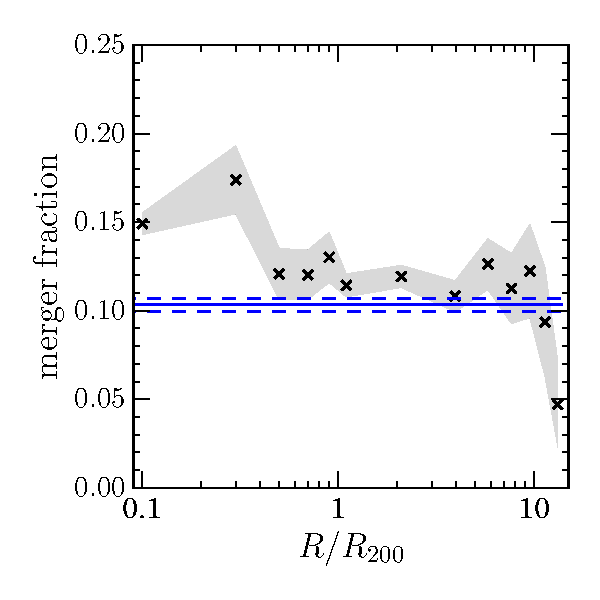
\includegraphics[width=0.46\textwidth]{environment/merger_fraction_trend_with_log_radius_compare_sat_field_cand.pdf}}
\caption[Merger fraction with group radius in the \textsc{gz2-group} sample]{Merger fraction in the \textsc{gz2-group} sample binned in projected group-centric radius, normalised by $R_{200}$, a proxy for the virial radius of a group. The shaded region shows $\pm1\sigma$ on the merger fraction. The merger fraction of the \textsc{gz2-sat-field} sample is also shown (blue solid line) with $\pm1\sigma$ (blue dashed line).}
\label{fig:mergerradius}
\end{figure}


I perform an initial sanity check on the \textsc{gz2-group} sample by recreating the morphology-density relation of \citet[][see Figure~\ref{fig:dressler}]{dressler80} in Figure \ref{fig:morphradius}, which shows the mean disc and smooth vote fractions as a function of group radius. The mean disc vote fraction decreases from the mean field value (blue line) within $1$ virial radius. Simultaneously, the mean smooth vote fraction increases, which is in agreement with previous studies on the morphology-density relation \citep{dressler80, smail97, poggianti99, postman05, Bamford09}. The extensive morphological classifications provided by GZ2 also allow for the investigation of how more detailed morphological structure is affected by the group environment.  

Figure \ref{fig:barradius} shows how the bar fraction (number of barred disc galaxies over the number of disc galaxies; see Section~\ref{sec:morphfrac}) increases significantly over the field fraction (blue solid line) with decreasing group-centric radius, in agreement with \cite{barazza09}. Figure \ref{fig:mergerradius} shows how the merger fraction does not significantly deviate from the field fraction (blue solid line) except for galaxies found within one virial radius. As discussed in Chapter~\ref{chap:agn}, mergers are thought to drive bulge growth and so similarly, Figure~\ref{fig:bulgeradius} shows how the fraction of galaxies with obvious/dominant bulges increases over the field value in the inner regions of the group (in agreement with \citealt{diaferio01}) and the fraction of those with none/just noticeable bulges decreases below the field value within $1$ virial radius. 

%Figure \ref{fig:sfrradius} shows how the SFR of the \textsc{gz2-group} sample does indeed decline with decreasing group-centric distance, significantly below the mean SFR of the \textsc{gz2-field} sample shown by the blue dashed line. This is in agreement with the results of \cite{gomez03} who observe a similar decline in SFR with group-centric radius in SDSS clusters (see for example, Figure 6 in \citealt{gomez03}). This coincides with the morphological fraction changes seen in Figures~\ref{fig:morphradius}-{\ref{fig:merger radius} in support of the conclusions of \citet{smethurst15} that quenching is morphologically dependent. 


%\begin{figure}
%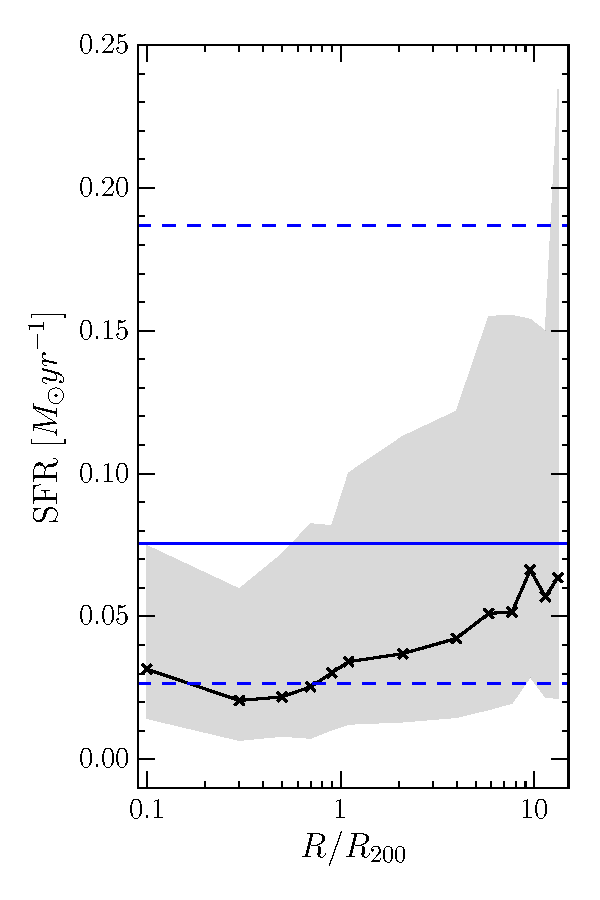
\includegraphics[width=0.46\textwidth]{environment/sfr_trend_with_log_radius_field_matched_blue_dashed_hlines_gomez_03_rv_not_r200.pdf}
%\caption{Median $H\alpha$ derived star formation rates of satellite galaxies in the \textsc{gz2-group} sample, binned in projected group-centric radius, normalised by $R_{200}$, a proxy for the virial radius of a group.  The shaded region shows the SFRs encompassed by $50\%$ of the population in a given bin. The median SFR of the \textsc{gz2-sat-field} sample is shown (blue solid line) along with the 25th and 75th percentiles (blue dashed lines).}
%\label{fig:sfrradius}
%\end{figure}

\subsection{Quenching histories in the group environment}\label{sec:resultssfhs}

\begin{figure*}
\centering{
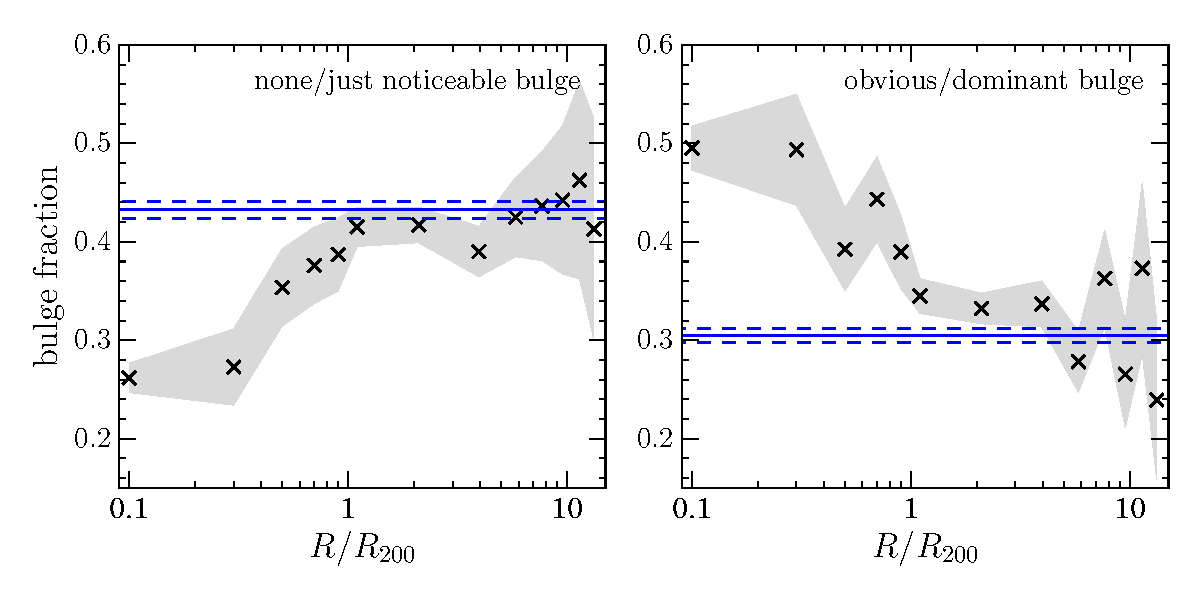
\includegraphics[width=0.85\textwidth]{environment/min_max_bulge_fraction_trend_with_log_radius_sat_field_cand.pdf}}
\caption[Bulge fraction with group radius in the \textsc{gz2-group} sample]{Fraction of galaxies with none/just noticeable bulge classifications (left) and with obvious/dominant bulge classifications (right) in the \textsc{gz2-group} sample binned in projected group-centric radius, normalised by $R_{200}$, a proxy for the virial radius of a group. The shaded regions shows $\pm1\sigma$ on the bulge fractions. The bulge fractions of the \textsc{gz2-sat-field} sample are also shown (blue solid lines) with $\pm1\sigma$ (blue dashed lines).}
\label{fig:bulgeradius}
\end{figure*}

\begin{figure}
\centering{
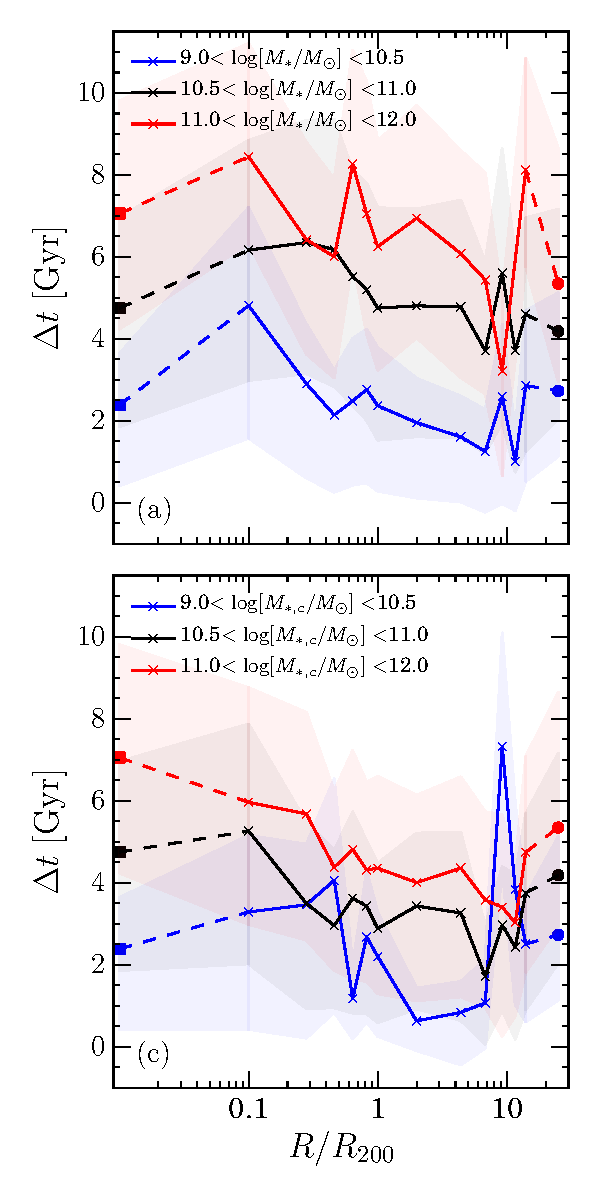
\includegraphics[width=0.48\textwidth]{environment/time_since_quenching_M*_Mh.pdf}
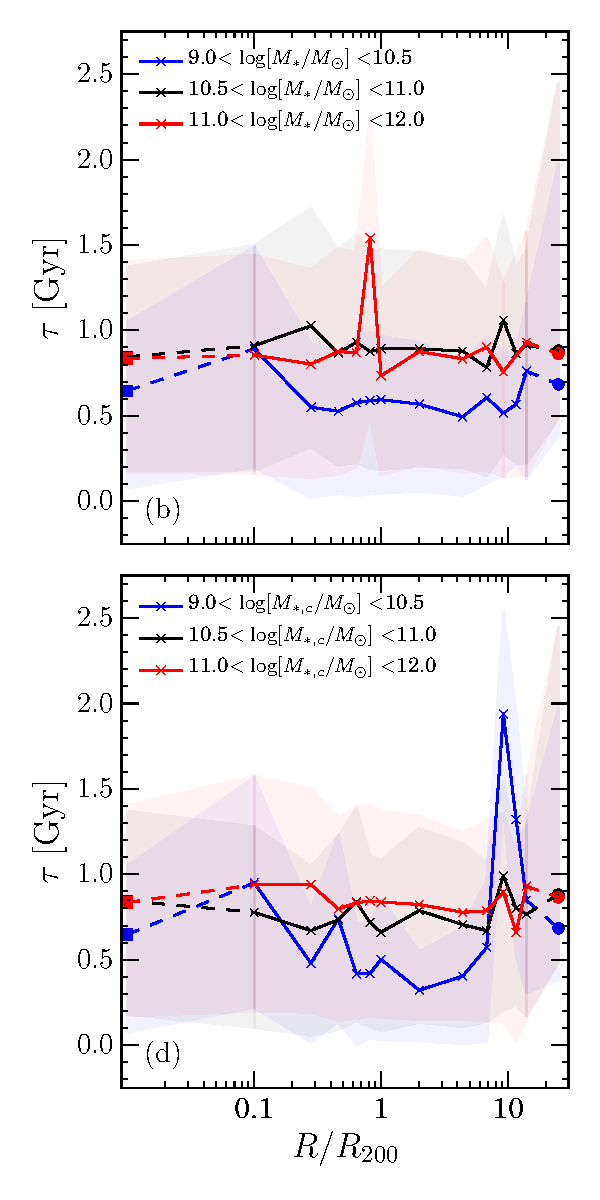
\includegraphics[width=0.48\textwidth]{environment/rate_of_quenching_M*_Mh.pdf}
\caption[Trend of $\Delta t$ and $\tau$ with group radius split by stellar mass and halo mass]{The time since quenching onset ($\Delta t = t_{obs} - t_{q}$; left) and rate of quenching ($\tau$; right) binned in group radius, $R/R_{200}$, for satellite galaxies (crosses) split into bins of stellar mass (top) and stellar mass of the corresponding central galaxy (bottom; a proxy for halo mass of a group). The corresponding values for central galaxies (squares, plotted at $\sim0.01 R/R_{200}$) and galaxies in the \textsc{gz2-cent-field-q} sample (circles, plotted at $25 R/R_{200}$) are shown and connected by the dashed lines to help guide the eye. The shaded regions show the $\pm1\sigma$ on $\Delta t$ and $\tau$ in each bin of $R/R_{200}$.}
\label{fig:timesinceradius}}
\end{figure}

\begin{figure}
\centering{
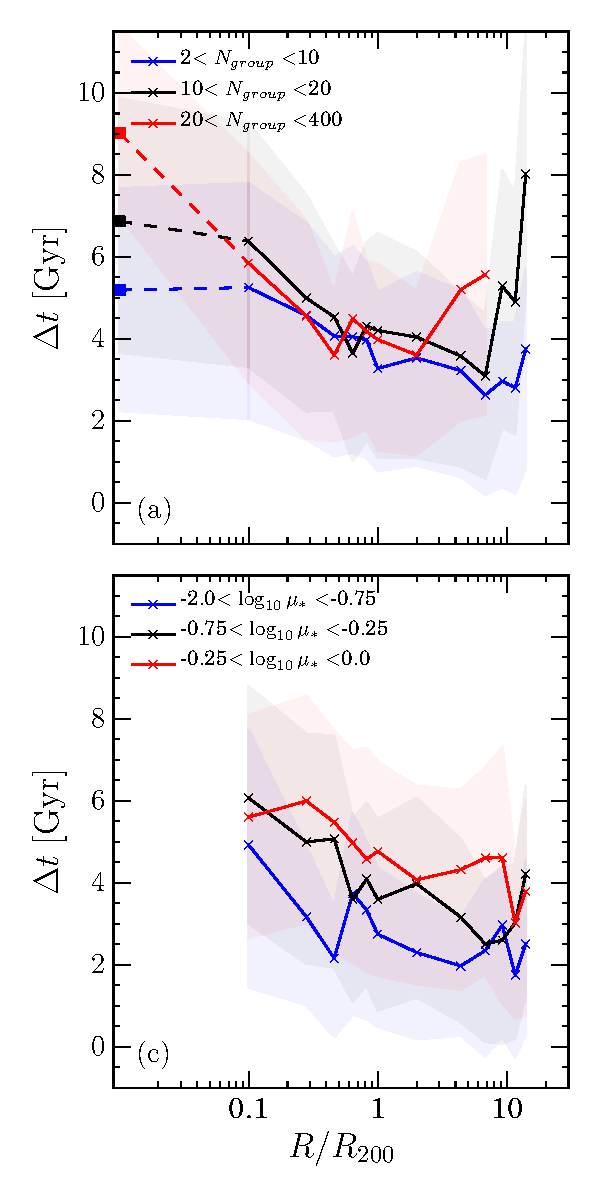
\includegraphics[width=0.48\textwidth]{environment/time_since_quenching_mu_Ngroup.pdf}
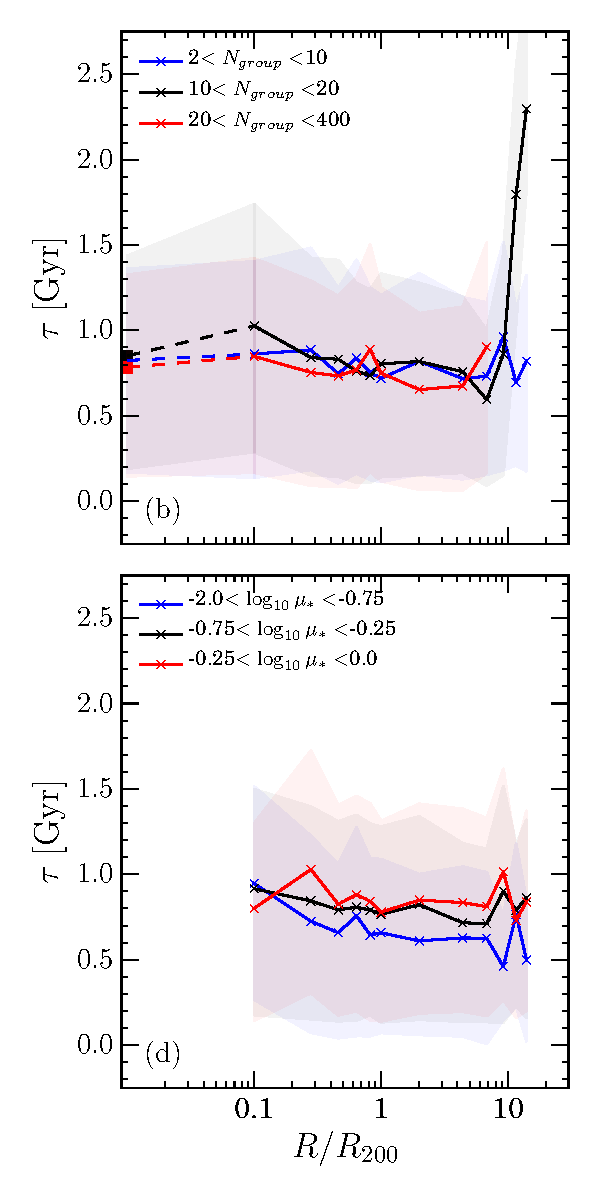
\includegraphics[width=0.48\textwidth]{environment/rate_of_quenching_mu_Ngroup.pdf}
\caption[Trend of $\Delta t$ and $\tau$ with group radius split by number in group and stellar mass ratio]{The time since quenching onset ($\Delta t = t_{obs} - t_{q}$) and rate of quenching ($\tau$; right) binned in group radius, $R/R_{200}$, for satellite galaxies (crosses) split into bins of stellar mass ratio ($\mu_* = M_*/M_{cent,*}$, top) and number of group members ($N_{group}$, bottom). The corresponding values for central galaxies (squares, plotted at $\sim0.01 R/R_{200}$) and galaxies in the \textsc{gz2-cent-field-q} sample (circles, plotted at $25 R/R_{200}$) are shown, where possible, and connected by the dashed lines to help guide the eye. The shaded regions show the $\pm1\sigma$ on $\Delta t$ and $\tau$ in each bin of $R/R_{200}$.}
\label{fig:timesinceradiusmu}}
\end{figure}

\begin{figure}
\centering{
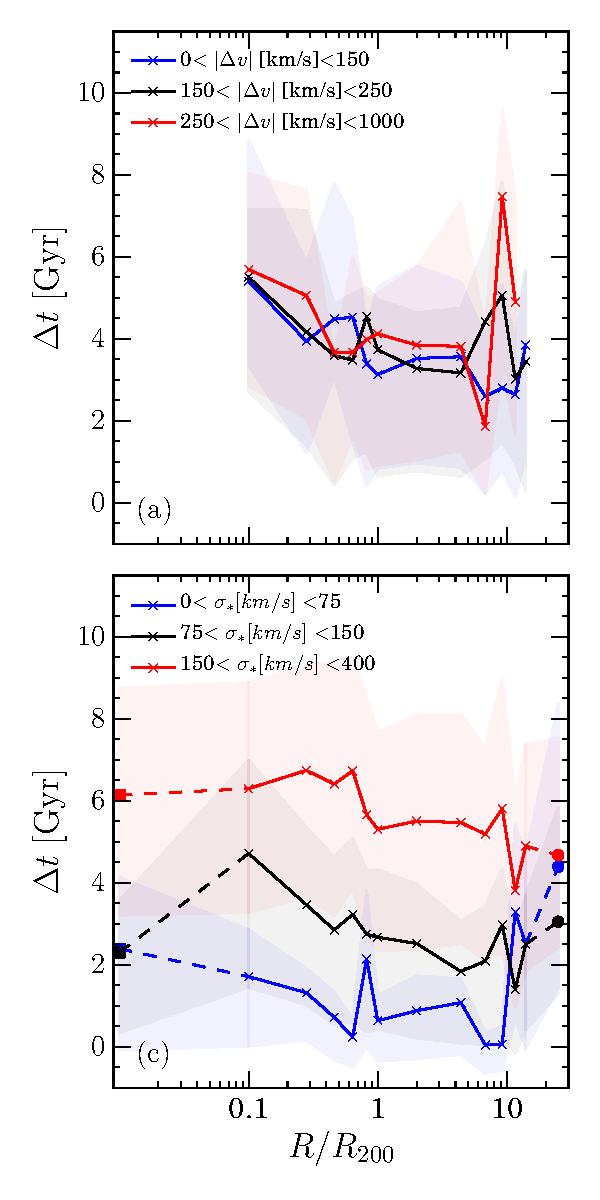
\includegraphics[width=0.48\textwidth]{environment/time_since_quenching_delv_sigma.pdf}
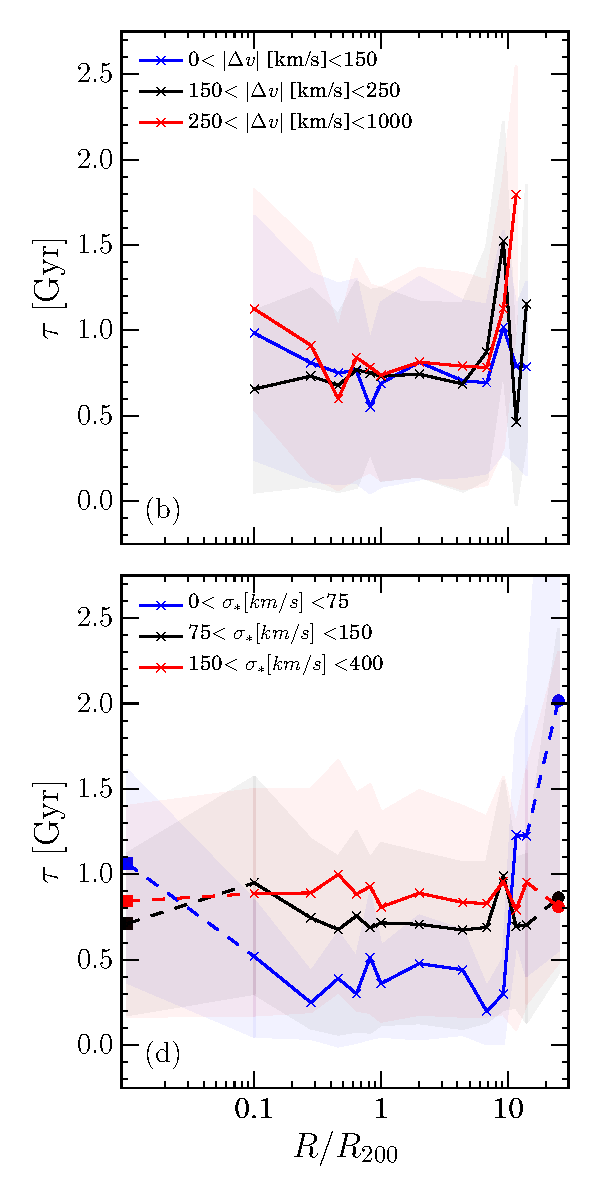
\includegraphics[width=0.48\textwidth]{environment/rate_of_quenching_delv_sigma.pdf}
\caption[Trend of $\Delta t$ and $\tau$ with group radius split by relative velocity and stellar velocity dispersion]{The time since quenching onset ($\Delta t = t_{obs} - t_{q}$; left) and rate of quenching ($\tau$; right) binned in group radius, $R/R_{200}$, for satellite galaxies (crosses) split by the absolute relative velocity of the satellite to its central galaxy ($|\Delta v|$, top) and stellar velocity dispersion ($\sigma_*$, bottom). The corresponding values for central galaxies (squares, plotted at $\sim0.01 R/R_{200}$) and galaxies in the \textsc{gz2-cent-field-q} sample (circles, plotted at $25 R/R_{200}$) are shown, where possible, and connected to the satellite values by the dashed lines to help guide the eye. The shaded regions show the $\pm1\sigma$ on $\Delta t$ and $\tau$ in each bin of $R/R_{200}$.}
\label{fig:timesinceradiusvel}}
\end{figure}

The SFHs of all galaxies in both the \textsc{gz2-group} and \textsc{gz2-cent-field-q} samples were analysed using \starpy, providing the posterior probability distribution across the two-parameter space for an individual galaxy.  Whereas in Chapters~\ref{chap:morph} \& \ref{chap:agn} the \textsc{popstarpy} method was then used to combine and weight the individual distributions to give an overall distribution representing the population of galaxies, in this study, no differences could be seen across the population densities in three bins of projected group-centric radius. In this Chapter, I instead take the 50th percentile walker position of an individual posterior probability distribution to give the most likely quenching time, $t_{q}$, and quenching rate, $\tau$, for each galaxy (shown by the solid blue lines in Figure~\ref{one_example}).

This simplifies the output from \starpy\ for each galaxy from a probability distribution to just two values, with $\pm1\sigma$ uncertainties (shown by the dashed blue lines in Figure~\ref{one_example}) which encompass the spread of the individual galaxy's SFH posterior probability distribution. In this Chapter I will calculate the time since quenching onset, $\Delta t$, for a given galaxy by calculating {\bf $\Delta t = t^\mathrm{obs} - t_{q}$} (where $t^{\rm{obs}}$ is the age of the Universe at a galaxy's observed redshift; see Section~\ref{qmod}). 

With the output from \starpy~ I can observe the trends in the time since quenching onset, $\Delta t$, and quenching rate, $\tau$, with group radius, $R/R_{200}$, for satellite galaxies and central galaxies in the \textsc{gz2-group} sample, compared with galaxies in the \textsc{gz2-cent-field-q} sample. This is shown in Figures \ref{fig:timesinceradius} - \ref{fig:timesinceradiusvel} wherein the \textsc{gz2-group} galaxies are binned by stellar mass (Figures~\ref{fig:timesinceradius}a-b), halo mass (Figures~\ref{fig:timesinceradius}c-d), mass ratio (Figures~\ref{fig:timesinceradiusmu}a-b), number of group galaxies (Figures~\ref{fig:timesinceradiusmu}c-d), relative velocity (Figures~\ref{fig:timesinceradiusvel}a-b) and stellar velocity dispersion (Figures~\ref{fig:timesinceradiusvel}c-d). All bin thresholds were chosen to give approximately the same number of galaxies in each bin. 

Across all the left panels in Figures~\ref{fig:timesinceradius} - \ref{fig:timesinceradiusvel} a general trend for increasing time since quenching onset with decreasing group radius can be seen. As in Figures \ref{fig:morphradius}$-$\ref{fig:bulgeradius} significant differences from the mean field values arise at radii less than one virial radius. However, no trend with group radius is seen for the rate at which quenching occurs for satellites in the \textsc{gz2-group} sample (right panels Figures~\ref{fig:timesinceradius} - \ref{fig:timesinceradiusvel}). This suggests that whatever mechanisms cause quenching in a group will do so at the same rate in both the dense inner and sparse outer regions. 

In Figure~\ref{fig:timesinceradius}a the \textsc{gz2-group} sample is split by stellar mass, $M_*$, and a clear trend for increasing $\Delta t$ with increasing stellar mass for satellite, central and field galaxies can be seen. However, this trend is less apparent for the rate of quenching seen in Figure~\ref{fig:timesinceradius}b. The central galaxies (shown by the square points) appear to have quenched more recently than the inner satellites (at $\sim0.1R/R_{200}$) of the same mass but have done so at the same quenching rate. 

In the bottom panels of Figure \ref{fig:timesinceradius} I split the \textsc{gz2-group} sample by halo mass by using the stellar mass of the corresponding central galaxy of a group, $M_{cent,*}$, as a proxy. I find a clear trend for increasing time since quenching onset with increasing halo mass for satellite, central and field galaxies (Figure~\ref{fig:timesinceradius}c) but once again this trend is less apparent for the rate of quenching (Figure~\ref{fig:timesinceradius}d) suggesting that the halo mass does not affect which quenching mechanism acts upon either central or satellite galaxies. 

To account for the effects of conformity, whereby satellites of higher mass tend to be found in higher mass halos \citep{weinmann06, kauffmann13, hearin15, hatfield16}, I also split the satellites of the \textsc{gz2-group} sample by the stellar mass ratio of the satellite to its central galaxy, $\mu_* = M_*/M_{cent,*}$, in the top panels of Figure~\ref{fig:timesinceradiusmu}. $\Delta t $ increases more steeply with group radius (particularly within $\sim$ one virial radius; Figure~\ref{fig:timesinceradiusmu}a) for satellite galaxies with much smaller masses than their group central ($-2.0 < \log_{10}\mu_* < -0.75$, shown by the blue curve). Once again this is not the case for the rate that quenching occurs, as shown in Figure~\ref{fig:timesinceradiusmu}b. 

Another property of the group which is expected to affect the satellite quenching histories is the number of group members, $N_{group}$, which should be roughly correlated with a satellite's local density in a  group. The bottom panels of Figure~\ref{fig:timesinceradiusmu} show that there is no trend with time since quenching onset or rate of quenching with increasing $N_{group}$ for satellite galaxies. The central galaxies (shown by the square points) however, do show a trend for increasing time since quenching as the number of group galaxies increases (Figure~\ref{fig:timesinceradiusmu}c), but the rate at which they quench is the same (Figure~\ref{fig:timesinceradiusmu}d) suggesting the mechanism by which this occurs is the same for all centrals regardless of halo mass. 

In the top panels of Figure \ref{fig:timesinceradiusvel} the \textsc{gz2-group} satellite galaxies are split into bins of their relative velocity to their central galaxies, i.e. the velocity at which they move through the dense group environment. There is no trend with either time since onset of quenching (Figure \ref{fig:timesinceradiusvel}a) or rate of quenching (Figure \ref{fig:timesinceradiusvel}b) with increasing relative velocity for galaxies in the \textsc{gz2-group} sample. This suggests that whatever quenching mechanism is occurring in groups, it is not correlated with the velocity at which satellites move through the dense environment.

The bottom panels of Figure~\ref{fig:timesinceradiusvel} show the trend with group radius for the \textsc{gz2-group} satellites when split into bins of galaxy stellar velocity dispersion $\sigma_*$ (note that this is not the velocity dispersion of the group) which is often used as a proxy for the galaxy potential. The stellar velocity dispersion shows the largest trend in $\Delta t$ (Figure~\ref{fig:timesinceradiusvel}c) for satellite galaxies across all right panels of Figures~\ref{fig:timesinceradius}-\ref{fig:timesinceradiusvel}, with galaxies with the smallest stellar velocity dispersions having quenched more recently. Although this trend is less apparent for the rate that quenching occurs when the satellite galaxies are split by $\sigma_*$ (Figure~\ref{fig:timesinceradiusvel}d), it is the largest trend seen across the right panels of Figures~\ref{fig:timesinceradius}-\ref{fig:timesinceradiusvel}. Also, field galaxies (shown by the circles at $\sim 25 R/R_{200}$) with low velocity dispersions are seen to quench at much slower rates than their satellite counterparts. This suggests that the rapid quenching observed for the low stellar velocity dispersion satellites is directly caused by the environment. 

The results shown in Figures~\ref{fig:timesinceradius}-\ref{fig:timesinceradiusvel} are summarised in Table~\ref{table:resultsum}.

\begin{table}[t]
\centering
\caption{Summary of results shown in Figures~\ref{fig:timesinceradius}-\ref{fig:timesinceradiusvel} denoting whether there is, $\checkmark$, or isn't, $\times$, a trend with $\Delta t$ when the \textsc{gz2-group} satellite galaxies are split by the stated property.}
\label{table:resultsum}
\begin{tabular*}{\textwidth}{l@{\extracolsep{\fill}}|cccccc}
\hline
\multicolumn{1}{r|}{}   & $M_*$    & $M_{\rm{cent},*}$ & $\mu_*$  & $N_{\rm{group}}$ & $|\Delta v|$ & $\sigma_*$ \\ \hline
Shown in Figure & \ref{fig:timesinceradius}a & \ref{fig:timesinceradius}c & \ref{fig:timesinceradiusmu}a & \ref{fig:timesinceradiusmu}c & \ref{fig:timesinceradiusvel}a & \ref{fig:timesinceradiusvel}c \\
Trend with $\Delta t$ when split by ...?~ & $\checkmark$ & $\checkmark$          & $\checkmark$ & $\times$         & $\times$     & $\checkmark$   \\ \hline
\end{tabular*}
\end{table}

\section{Discussion}\label{sec:disc}

I shall now consider the results presented in Section~\ref{sec:results} in the context of possible quenching mechanisms which could be responsible. 

\subsection{The role of mergers as quenching mechanisms in the group environment}\label{sec:rolemergerenv}

The merger classification in GZ2 has been shown to preferentially identify major mergers \citep{Darg10a}; while bulge formation in disc galaxies is often associated with evolutionary histories driven by minor mergers \citep{Croton06, tonini16}.  Although we see evidence for an enhanced merger fraction in the inner regions of the group environment in Figure~\ref{fig:mergerradius}, the bulge fractions in Figure~\ref{fig:bulgeradius} vary much more significantly from the field value than the merger fraction. This suggests that minor mergers may be more dominant than major mergers for satellites in the group environment, particularly at $R/R_{200} > 0.5$. 

If mergers are a dominant evolutionary mechanism for satellite galaxies, as the morphological evidence in Figures~\ref{fig:mergerradius} \& \ref{fig:bulgeradius} suggests, we would expect to see a difference in the quenching histories of satellites residing in groups with a larger number of members. However, the bottom panels of Figure \ref{fig:timesinceradiusmu} show that there is no trend with time since quenching onset or rate of quenching with increasing $N_{group}$ for the satellite galaxies. This suggests that mergers are not the dominant quenching mechanism for satellite galaxies, but that whatever mechanism is the cause of the quenching occurs at the same rate irrespective of group size. 

Central galaxies however, do show a trend for increasing time since quenching with increasing $N_{group}$ (square points in Figure \ref{fig:timesinceradiusmu}c) occurring at a rate of $\tau \sim 1 \rm{Gyr}$ (which as discussed in Chapter~\ref{chap:morph}, was attributed to mergers and galaxy interactions which could transform a galaxy's morphology). Therefore, the larger the number of group members, the more likely a central galaxy has a history dominated by mergers. This is in agreement with the findings of \citet{lin10}, \citet{ellison10}, \citet{lidman13} and \citet{mcintosh08}. The latter found, by studying a sample of local groups and clusters, that half of the mergers they identified involved the central galaxy. \cite{liu09} also found that the fraction of merging centrals increases with the richness of a cluster (a measure of the number of galaxies within $1\rm{h}^{-1}\rm{Mpc}$ of the central galaxy).

This idea is supported by the result in Figure~\ref{fig:timesinceradius}a showing that centrals of a given mass have quenched more recently than the inner satellites (at $\sim0.1R/R_{200}$) of a given mass. This suggests that an episode of more recent star formation, such as a starburst, may have occurred in the central galaxies but not in the inner satellites. Mergers are thought to cause an energetic burst of star formation which can in turn quench the remnant galaxy \citep[][as discussed in Section \ref{rapid}]{hopkins05, treister12, pontzen16}. This result is also suggestive of a merger dominated history for central galaxies but not for satellite galaxies.

\subsection{The role of mass quenching in the group environment}\label{sec:rolemassenv}

A trend is seen for increasing time since quenching with increasing stellar mass and velocity dispersion (a proxy for galaxy potential) for centrals, satellites and field galaxies in Figure~\ref{fig:timesinceradius}a and Figure~\ref{fig:timesinceradiusvel}c respectively. This is suggestive of mass quenching occurring across the entire galaxy population irrespective of environmental density, supporting the work of \citet{peng10, peng12, Gabor10} and \citet{darvish16}.

\subsection{The role of morphological quenching in the group environment}\label{sec:rolemorphenv}

The increasing bar fraction toward the central group regions  shown in Figure \ref{fig:barradius} \citep[in agreement with][]{skibba12}, suggests that bars may be partly responsible for the relation between quenched fraction and environmental density. This is consistent with findings that show that bars themselves may be the cause of morphological quenching through the funnelling of gas toward the central regions of galaxies \citep{athanassoula92b, sheth05} which is then used in star formation, exhausting the available gas\footnote{The gas which is funnelled to the centre by the bar may also be used to fuel an AGN. The AGN-environment connection has been extensively studied with conflicting results; \cite[e.g. see][]{miller03, pimbblet12, pimbblet13, elhert14, desouza16}. I attempted to study this in this investigation. However, only 204 satellites and 128 centrals of the \textsc{gz2-group} sample were identified as obscured Type 2 AGN using a BPT diagram. These low numbers of AGN mean that when split into bins of group radius we are well and truly dancing precariously on the low number statistics volcano and so no robust conclusions can be drawn.} (see Section~\ref{sec:morphquench}).

%As discussed in Chapter~\ref{chap:agn}, an inflow due to a bar may also be able to fuel an AGN. The AGN-environmental connection has been extensively studied with conflicting results; \cite{pimbblet13}, with optically selected AGN, and \cite{elhert14}, with X-ray selected AGN, showed that the AGN fraction decreases towards the inner regions of groups. However, these studies did not take into account the morphology-density relation of satellite galaxies, where bulge dominated galaxies dominate in the inner regions of groups. \cite{miller03} and more recently \cite{desouza16}, using a hierarchical Bayesian method, showed with optically selected AGN that although the AGN fraction decreases with group radius for early-type galaxies, it stays constant with group radius for late-types. This suggests that disc galaxies are still able to fuel their AGN even in dense environments, perhaps due to the enhanced bar fraction in the inner regions of the group.

We must therefore consider whether the environment itself may play a role in triggering the disk instabilities which can produce a bar. Indeed harassment and tidal interactions, believed to be common in the group environment, have been shown to both promote and inhibit bar formation dependent on the stellar mass \citep{noguchi88, moore96, skibba12}.  If the environment was indeed triggering a bar, then morphological quenching would be occurring in the group environment but indirectly due to environmental quenching. This suggests that the polarity between internal secular processes (`nature') and external environmental processes (`nurture') may not be as extreme as first thought, in agreement with \cite{skibba12}. 

\subsection{The role of the environment in quenching}\label{sec:roleenv}

Across all panels of Figures~\ref{fig:timesinceradius}-\ref{fig:timesinceradiusvel} a trend for increasing time since quenching onset with decreasing group radius is present. I interpret this as environmentally driven mechanisms causing quenching at the same rate throughout the infall time of a galaxy in a group. Galaxies which are now closer in fell into the group earlier and as they did so they started to quench, giving rise to a larger inferred $\Delta t$.

More massive halos are seen to have a greater impact on the star formation histories of their satellites than less massive halos in Figure~\ref{fig:timesinceradius}c. The halo mass is correlated with both (i) the gravitational potential of the group and (ii) the temperature of the IGM, suggesting that an environmental quenching mechanism which is correlated with one or both of these properties is responsible for this result.

Higher mass halos have hotter intra group medium (IGM) temperatures \citep{shimizu03, delpopolo05} which can have a greater impact on a galaxy through ram pressure stripping (RPS) of cold gas. \cite{gunngott72} define the ram pressure as:
\begin{equation}\label{eq:rps}
\rho_{\rm{IGM}}\cdot v^2 = 2\pi G \cdot \sigma_*(R) \cdot \sigma_g(R),
\end{equation}
where $\rho_{\rm{IGM}}$ is the density of the IGM, $\sigma_*(R)$ the star surface density, $\sigma_g(R)$ the gas surface density of the galaxy disc and $v$ the velocity of the galaxy through the IGM. Therefore if RPS is indeed a dominant environmental quenching mechanism we should see a trend in $\Delta t$ with the velocity of a satellite relative to its central galaxy.  However in Figure \ref{fig:timesinceradiusvel}a we see that this is not the case. This therefore rules out RPS as the dominant environmental quenching mechanism, in support of the simulations of \citet{emerick16, fillingham16} which showed that RPS could only remove $40-60\%$ of a satellite's gas.However, this conclusion may be due to the stellar mass range spanned by the \textsc{gz2-group} satellite galaxies which all have $M_* \geq 10^9 \rm{M}_{\odot}$, as simulations by \cite{fillingham16} suggest that RPS only becomes effective in lower mass satellites with $M_* \leq 10^{8-9} \rm{M}_{\odot}$, in agreement with \cite{hester06}. 

Above this mass threshold in the simulations of \cite{fillingham16}, a `starvation' (or strangulation) mode \citep{larson80, balogh00} dominantes, where a galaxy's extended gaseous halo is removed causing a quench, as cold gas for use in star formation can no longer be fed from the extended halo. This idea is supported by observations by \citet{peng10} which show that strangulation is a dominant mechanism for galaxies with $M_* < 10^{11}~M_{\odot}$ with a quenching timescale of $4~\rm{Gyr}.$ Such a mechanism will be correlated with the galaxy potential, as galaxies with a lower potential will be most easily stripped of their halos. This is apparent in Figure~\ref{fig:timesinceradiusvel}d where satellites with lower velocity dispersion (a proxy for the galaxy potential) are more rapidly quenched than their higher velocity dispersion counterparts and those in the field. Such a starvation mechanism is also correlated with halo mass, for which similar trends in $\Delta t$ are seen in Figure~\ref{fig:timesinceradius}c. The dominant environmental quenching mechanism occurring in the group environment must therefore be correlated with the group potential. This suggests that satellite galaxies may be most affected by gravitationally driven environmental effects, such as starvation, thermal evaporation of the galaxy halo and galaxy harassment. 


We can calculate an infall timescale for the satellite galaxies in the \textsc{gz2-group} sample if we assume that galaxies begin their infall into a group at a radius of $\sim10\rm{R}_{200}$ and stop infalling at $\sim0.1\rm{R}_{200}$\footnote{This assumes that galaxies will then merge with their central galaxy, however it is more likely that the satellite has a close pass with the central before it `backsplashes' into the group. See, for example, \cite{pimbblet11}.}. The difference in the time since quenching onset, $\Delta t$, between these two locations in a group will provide an estimate for how long it takes a satellite to infall. This assumes (i) that the galaxy starts to quench immediately when it enters the group and (ii) that the same environmentally driven quenching process is the only quenching mechanism affecting the satellites throughout their infall. I will define this property as $\delta \Delta t = \Delta t_{0.1R_{200}} - \Delta t_{10 R_{200}}$. In Figure~\ref{fig:timesinceradiusmu}c the trend seen in $\Delta t$ with group radius is the same regardless of the number of galaxies in the group, so this gives us an estimate for the average $\Delta t$ in each group-centric radius bin across the satellite population. I therefore estimate an average infall time of $\delta \Delta t \sim 3 ~\rm{Gyr}$ for the \textsc{gz2-group} satellites. The rate of quenching occurring across the group radius in Figure~\ref{fig:timesinceradiusmu}d is $\tau \sim 1~\rm{Gyr}$ (this is within the range of quenching rates theorised to cause a morphological change in Section~\ref{gv}) and so we can also estimate the average quenching timescale (i.e. the time taken to fully quench from the SFS to $5\sigma$ below the SFS, as in Chapters~\ref{chap:morph} \& \ref{chap:agn}) to be $\sim 4~\rm{Gyr}$ for the \textsc{gz2-group} satellites.

This infall time and quenching timescale are in agreement with the estimates of \cite{wetzel13} who used a high resolution cosmological N-body simulation to track satellite galaxy orbits in SDSS groups and clusters and found quenching timescales of $2-6~\rm{Gyr}$. Using a similar method, \cite{oman16} derive an infall time of $\sim4~\rm{Gyr}$ and quenching timescales between $4-6~\rm{Gyr}$ for galaxies in the mass range of the \textsc{gz2-group} sample. Similarly, \cite{hahn16} derive a total quenching timescale of $\sim4~\rm{Gyr}$ for satellite galaxies on infall into the group environment. However, the simulations by \cite{fillingham16} and \cite{emerick16} have shown that RPS cannot remove enough gas mass to completely quench a galaxy within $\sim2~\rm{Gyr}$ but can assist in reducing the starvation timescale so that galaxies can be quenched within the $\sim4~\rm{Gyr}$ quenching timescale calculated in this study. This suggests that although the effects of mechanisms correlating with the group potential are detectable in the quenching parameters of the \textsc{gz2-group} sample, this is only made possible by the constantly present, but less dominant effects of ram pressure stripping. 

This conclusion, along with that in Section~\ref{sec:rolemorphenv} where I noted that morphological quenching may only be present in the group environment due to the influence of the environment itself, suggests that all the mechanisms discussed here will affect a galaxy which is infalling through the group environment at some point in its lifetime. A single mechanism may be more dominant in the evolution of an individual galaxy but to achieve the correlations between morphology, colour and quenched galaxy fraction with density observed across the entire population all mechanisms need to act in concert.  

\section{Conclusions}\label{sec:conc}

Using the \citet{berlind06} group catalogue, I have constructed a sample of group galaxies in the SDSS which were cross matched with Galaxy Zoo 2 and GALEX in order to determine their most likely SFHs using \starpy. I have shown that although mass quenching, morphological quenching and mergers are all important mechanisms at work in quenching the galaxies in the group environment, the environment does play a role in quenching galaxies as they infall into the group. I have discussed the possibility that no single mechanism will dominate across the group population, with all mechanisms acting collaboratively. My findings are summarised as follows:
\begin{enumerate}[(i)]
\item The bar, obvious bulge and merger fractions are all seen to increase above the field value in the inner regions of the groups of the \textsc{gz2-group} sample in Figures~\ref{fig:barradius}, \ref{fig:bulgeradius} \& \ref{fig:mergerradius} respectively.  
 
\item Mergers are the dominant quenching mechanism for central galaxies but not for satellite galaxies. Satellites may undergo a minor merger in the group environment but their effects are only discernible by their indirect effect on the bulge fraction (see Figure~\ref{fig:bulgeradius}).
 
\item Mass quenching is occurring across the entire \textsc{gz2-group} sample for centrals and satellites irrespective of the environmental density (see Figure~\ref{fig:timesinceradius}a).
 
\item Morphological quenching is occurring for \textsc{gz2-group} satellite galaxies as evidenced by the heightened bar fraction in the inner group regions (see Figure~\ref{fig:barradius}). However, this may be indirectly due to environmental quenching since galaxy interactions and harassment are believed to be able to trigger bars. This suggests the polarity between `nature' vs. `nurture' may not be as extreme as previously thought. 

\item The environment does cause quenching across the \textsc{gz2-group} sample, as evidenced by the increase in the time since quenching with decreasing group radius seen across all left panels of Figures~\ref{fig:timesinceradius}-\ref{fig:timesinceradiusvel}. The results in Figures \ref{fig:timesinceradius}a \&  \ref{fig:timesinceradiusvel}c suggest that this is caused by a quenching mechanism correlated with the group potential, such as harassment, interactions and starvation, rather than the velocity of a satellite through the group, such as ram pressure stripping. This quenching occurs within an average quenching timescale of $\sim4~\rm{Gyr}$ from star forming to complete quiescence, after an average infall time of $\sim 3 ~\rm{Gyr}$. 
  
It is apparent from the results presented in this Chapter that many quenching mechanisms are all occurring simultaneously in the group environment; therefore a superposition of all of the effects of these mechanisms is seen in the quenching histories of the \textsc{gz2-group} sample, which in turn gives rise to the morphology-density relation observed. 
 
  
\end{enumerate}
